% DO NOT COMPILE THIS FILE DIRECTLY!
% This is included by the other .tex files.

\begin{frame}[t,plain]
\titlepage
\end{frame}

\begin{frame}
 \frametitle{MISP and Starting from a Practical Use-Case}
 \begin{itemize}
         \item In 2012, during a malware analysis workgroup, we realized that multiple analysts were working independently on the same malware.
         \item To streamline our efforts and avoid redundancy, we sought a {\bf method for easy and automated information sharing}.
         \item Christophe Vandeplas, then employed at the Belgian Ministry of Defense, presented his preliminary work on what would eventually evolve into the MISP platform.
         \item An initial version of the MISP platform was adopted by the MALWG, and the valuable feedback from users fueled further development and enhancements.
         \item Today, MISP has grown into a platform driven by {\bf community development}.
 \end{itemize}
\end{frame}

\begin{frame}
\frametitle{about CIRCL}
    The Computer Incident Response Center Luxembourg (CIRCL)\footnote{\url{https://www.circl.lu/}} is a government-driven initiative designed to provide a systematic response facility to computer security threats and incidents. CIRCL is the CERT for the private sector, communes and non-governmental entities in Luxembourg and is operated by Luxembourg House of Cybersecurity (LHC) g.i.e.
\end{frame}

\begin{frame}
\frametitle{MISP and CIRCL}
\begin{itemize}
    \item CIRCL is mandated by the Ministry of Economy and acting as the Luxembourg National CERT for private sector (under the NIS directive).
\item CIRCL leads the development of the Open Source MISP threat intelligence platform which is used by many military or intelligence communities, private companies, financial sector, National CERTs and LEAs globally.
\item {\bf CIRCL runs multiple large MISP communities performing active daily threat-intelligence sharing}.
\end{itemize}
        
\includegraphics{en_cef.png}
\end{frame}

\begin{frame}
    \frametitle{What is MISP? (core software)}
\begin{itemize}
       \item MISP is a {\bf threat information sharing} platform that is free \& open source software
       \item A tool that {\bf collects} information from partners, your analysts, your tools, feeds
       \item Normalises, {\bf correlates}, {\bf enriches} the data
       \item Allows teams and communities to {\bf collaborate}
       \item {\bf Feeds} automated protective tools and analyst tools with the output
\end{itemize}
\end{frame}

\begin{frame}
        \frametitle{MISP Project Overview}
        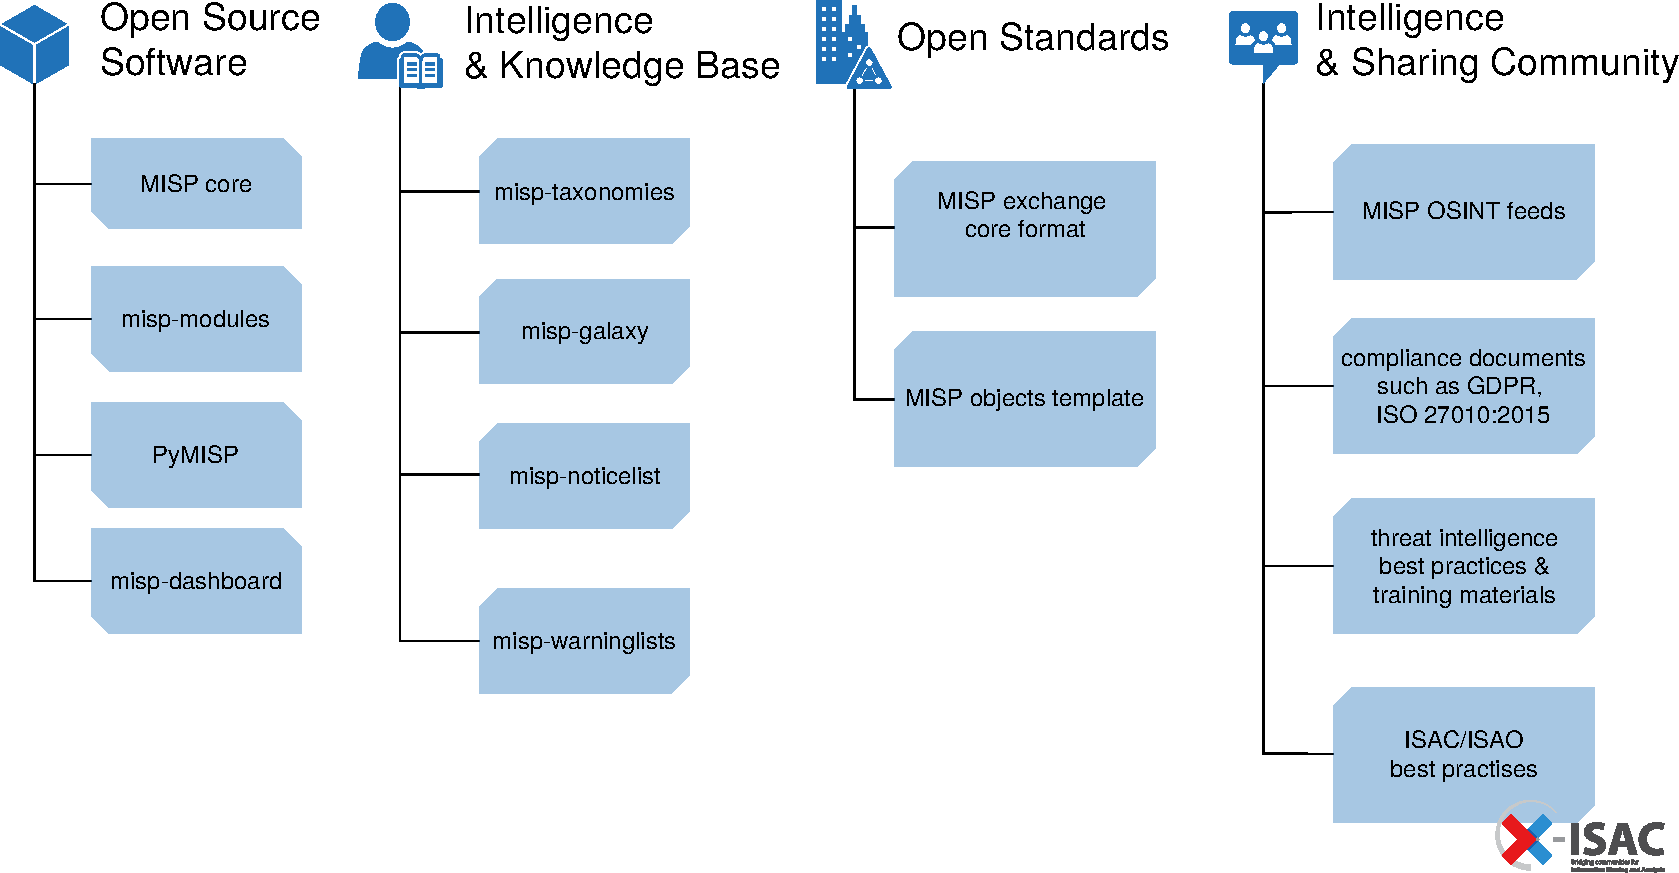
\includegraphics[scale=0.35]{misp-overview-simplified.pdf}
\end{frame}

\begin{frame}
\frametitle{Development based on practical user feedback}
\begin{itemize}
\item There are many different types of users of an information sharing platform like MISP:
        \begin{itemize}
                \item {\bf Malware reversers} willing to share indicators of analysis with respective colleagues.
                \item {\bf Security analysts} searching, validating and using indicators in operational security.
                \item {\bf Intelligence analysts} gathering information about specific adversary groups.
                \item {\bf Law-enforcement} relying on indicators to support or bootstrap their DFIR cases.
                \item {\bf Risk analysis teams} willing to know about the new threats, likelyhood and occurences.
                \item {\bf Fraud analysts} willing to share financial indicators to detect financial frauds.
        \end{itemize}
\end{itemize}
\end{frame}

%\begin{frame}
%\frametitle{MISP model of governance}
%\begin{center}
%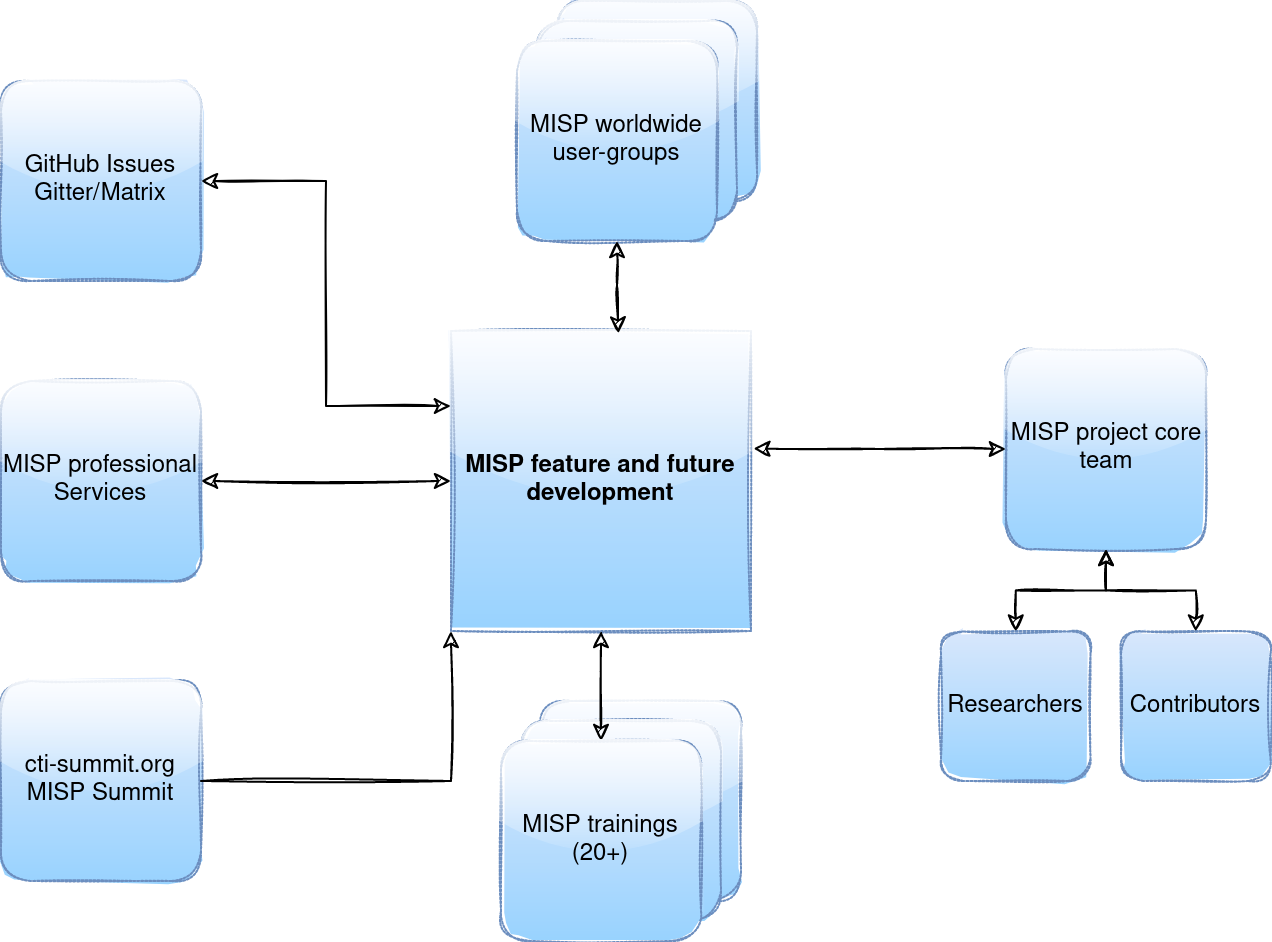
\includegraphics[scale=0.2]{governance.png}
%\end{center}
%\end{frame}

\begin{frame}
\frametitle{Many objectives from different user-groups}
        \begin{itemize}
                \item Sharing indicators/selectors for a {\bf detection} matter.
                        \begin{itemize}
                                \item 'Do I have infected systems in my infrastructure or the ones I operate?'
                        \end{itemize}
                \item Sharing indicators to {\bf block}.
                        \begin{itemize}
                                \item 'I use these attributes to block, sinkhole or divert traffic.'
                        \end{itemize}
                \item Sharing indicators to {\bf perform intelligence}.
                        \begin{itemize}
                                \item 'Gathering information about campaigns and attacks. Are they related? Who is targeting me? Who are the adversaries?'
                        \end{itemize}
                \item $\rightarrow$ These objectives can be conflicting (e.g. False-positives have different impacts)
        \end{itemize}
\end{frame}

\begin{frame}
 \frametitle{Communities using MISP}
 \begin{itemize}
	 \item Communities are groups of users sharing within a set of common objectives/values.
	 \item CIRCL operates multiple MISP instances with a significant user base (more than 1200 organizations with more than 4000 users).
         \item {\bf Trusted groups} running MISP communities in island mode (air gapped system) or partially connected mode.
	 \item {\bf Financial sector} (banks, ISACs, payment processing organizations) use MISP as a sharing mechanism.
	 \item {\bf Military and international organizations} (NATO, military CSIRTs, n/g CERTs,...).
	 \item {\bf Security vendors} running their own communities (e.g. Fidelis) or interfacing with MISP communities (e.g. OTX).
         \item {\bf Topical communities} set up to tackle individual specific issues (COVID-19 MISP)
 \end{itemize}
\end{frame}

\begin{frame}
  \frametitle{NATO and MISP Communities}
  \begin{center}
      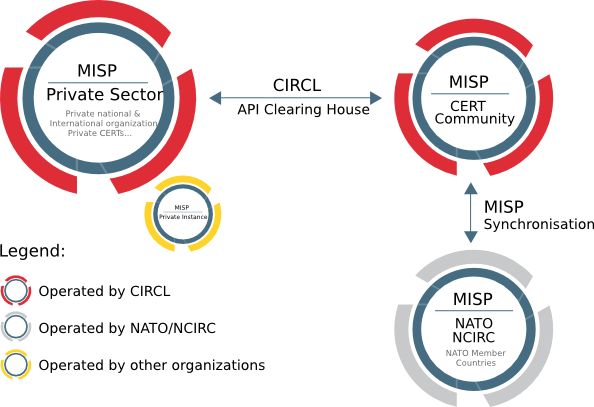
\includegraphics[scale=0.5]{misp-flows.png}
  \end{center}
\end{frame}

\begin{frame}
  \frametitle{Evolving Military Use Cases with MISP}
  \begin{itemize}
      \item MISP's versatile standard\footnote{\url{https://www.misp-standard.org/}} seamlessly integrates with military protocols, enhancing interoperability.
      \item Supports diverse intelligence inputs, including {\bf HUMINT} (Human Intelligence), {\bf SIGINT} (Signals Intelligence), and {\bf OSINT} (Open Source Intelligence), within the MISP framework.
  \end{itemize}                                                                                                                                             
\end{frame}

\begin{frame}
    \frametitle{SIGINT - MISP Integration with SigMF}
  \begin{itemize}
      \item MISP has added support for the Signal Metadata Format Specification (SigMF)\footnote{\url{https://www.misp-project.org/2023/08/23/MISP_now_supports_Signal_Metadata_Format_Specification_SigMF.html/}}, used widely in {\bf software-defined radio and signal processing}.
    \item New SigMF-related object templates introduced:
      \begin{itemize}
        \item SigMF Recording
        \item SigMF Archive
        \item SigMF Expanded Recording
      \end{itemize}
    \item Enrichment features in MISP allow expansion of SigMF recordings, aiding in data analysis and integration of signal metadata into MISP attributes.
    \item This integration facilitates improved search capabilities and data analysis within MISP.
  \end{itemize}
\end{frame}

\begin{frame}
    \frametitle{SIGINT - MISP Integration with SigMF}
\begin{center}
    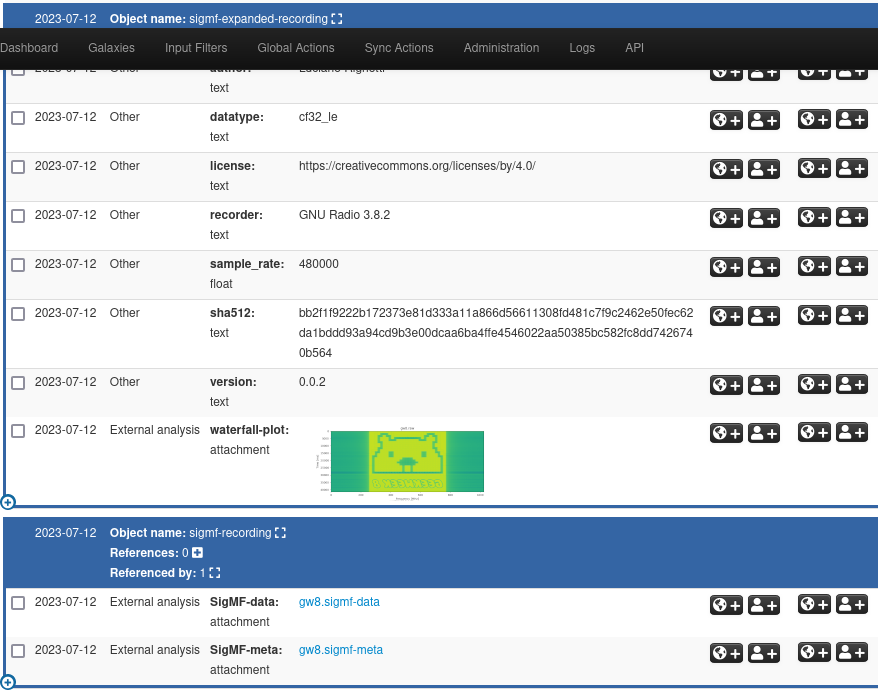
\includegraphics[scale=0.3]{waterfall.png}
\end{center}
\end{frame}

\begin{frame}
    \frametitle{HUMINT - MISP Versatile Objects}
    \begin{itemize}
        \item The MISP standard is extensible; objects can be easily created to cover specific use cases.
        \item Military organizations often have their own unique data models.
        \item The MISP standard includes 344\footnote{\url{https://www.misp-project.org/objects.html}} default object templates, many of which are applicable to HUMINT.
    \end{itemize}
\end{frame}

\begin{frame}
    \frametitle{HUMINT - MISP versatile objects}
\begin{center}
    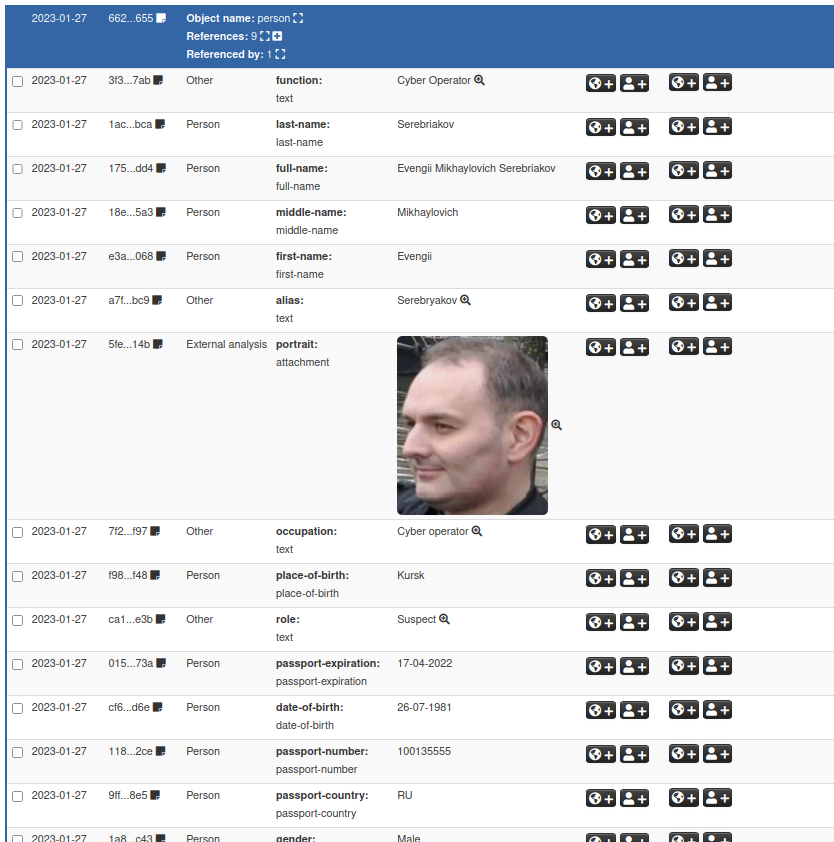
\includegraphics[scale=0.3]{gru-1.png}
\end{center}
\end{frame}

\begin{frame}
    \frametitle{Attribution and Threat Actors}
\begin{itemize}
       \item MISP includes a default knowledge base known as MISP Galaxies\footnote{\url{https://www.misp-galaxy.org/}},
       \item For instance, the Threat Actor galaxy contains an officially maintained list of Threat Actors.
       \item Military organizations often have their own methods of attribution or adaptations from existing models.
       \item MISP allows users to fork and maintain their own perspectives on threat actors.                                       
\end{itemize}
\end{frame}

\begin{frame}
\frametitle{Sharing in MISP}
    \begin{itemize}
        \item Sharing via distribution lists - {\bf Sharing groups}
        \item {\bf Delegation} for pseudo-anonymised information sharing
        \item {\bf Proposals} and {\bf Extended events} for collaborated information sharing
        \item Synchronisation, Feed system, air-gapped sharing
        \item User defined {\bf filtered sharing} for all the above mentioned methods
        \item Cross-instance information {\bf caching} for quick lookups of large data-sets
        \item Support for multi-MISP internal enclaves
    \end{itemize}
\end{frame}


\begin{frame}
\frametitle{Information quality management}
    \begin{itemize}
        \item Correlating data
        \item Feedback loop from detections via {\bf Sightings}
        \item {\bf False positive management} via the warninglist system
        \item {\bf Enrichment system} via MISP-modules
        \item {\bf workflow} system to review and control information publication
        \item {\bf Integrations} with a plethora of tools and formats
        \item Flexible {\bf API} and support {\bf libraries} such as PyMISP to ease integration
        \item {\bf Timelines} and giving information a temporal context
        \item Full chain for {\bf indicator life-cycle management}
    \end{itemize}
\end{frame}

\begin{frame}
        \frametitle{Conclusion}
        \begin{itemize}
                \item \textbf{Information sharing practices are derived from usage} and exemplified through learning by imitation from shared information.
                \item MISP is fundamentally a tool. The key is your sharing and analyst practices, which should find the tool transparent and supportive.
                \item Enable military users to customize MISP to meet their community's specific use cases.                                                                     
                \item The MISP project combines open-source software, open standards, best practices, and communities to facilitate effective information sharing.
        \end{itemize}
\end{frame}


